
% Risk Tolerance.
\section{Risk Tolerance}

\begin{figure}[!h]
\centering
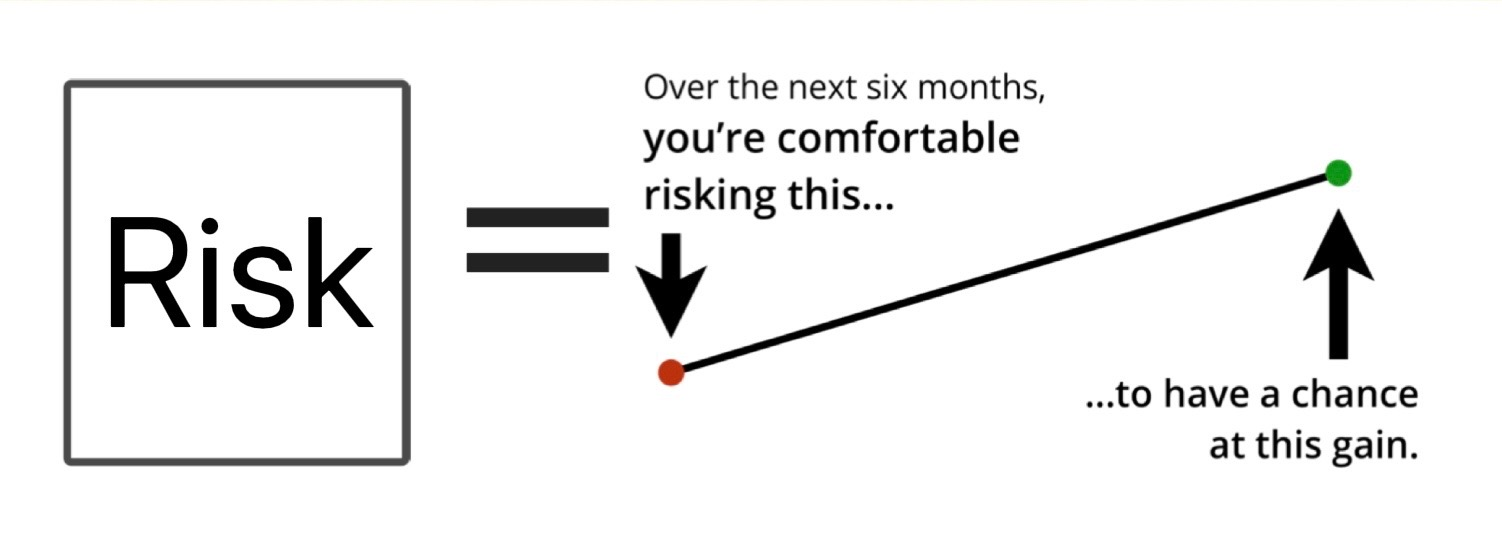
\includegraphics[width=0.7\textwidth]{./Figures/Tolerance.PNG}
\caption{The Risk Tolerance.}
\end{figure}

The risk tolerance describes the risk-resistance capacity of our client. According to the demand of our client. Our goal for this 6-month period of the investment is to minimise the risk, and to maximise the return under this minimum risk condition.

The Risk can be closely approximated by the variance of the return of the investment portfolio. To minimise the risk, we aim to minimise the variance of the returns of the investment portfolio. The variance is given by 

$$
\begin{aligned}
\operatorname{Var}\left[\sum_{i=1}^{15} \tilde{r}_{i} x_{i}\right] 
&=\sum_{i=1}^{15} \sum_{j=1}^{15} x_{i} x_{j} \sigma_{i j}
\end{aligned}
$$
where $\sigma_{i j}$ is the covariance of the return of stock $i$ with stock $j$.



%突然发现一个问题 我们算出来的数据 都是以一年为准的吧-你这个是说的哪个啊
%然而我们要算的是六个月以内的return 和risk? 所以return rate和risk rate会有变化吗
%看眼微信